\begin{figure}[h]
    \centering
    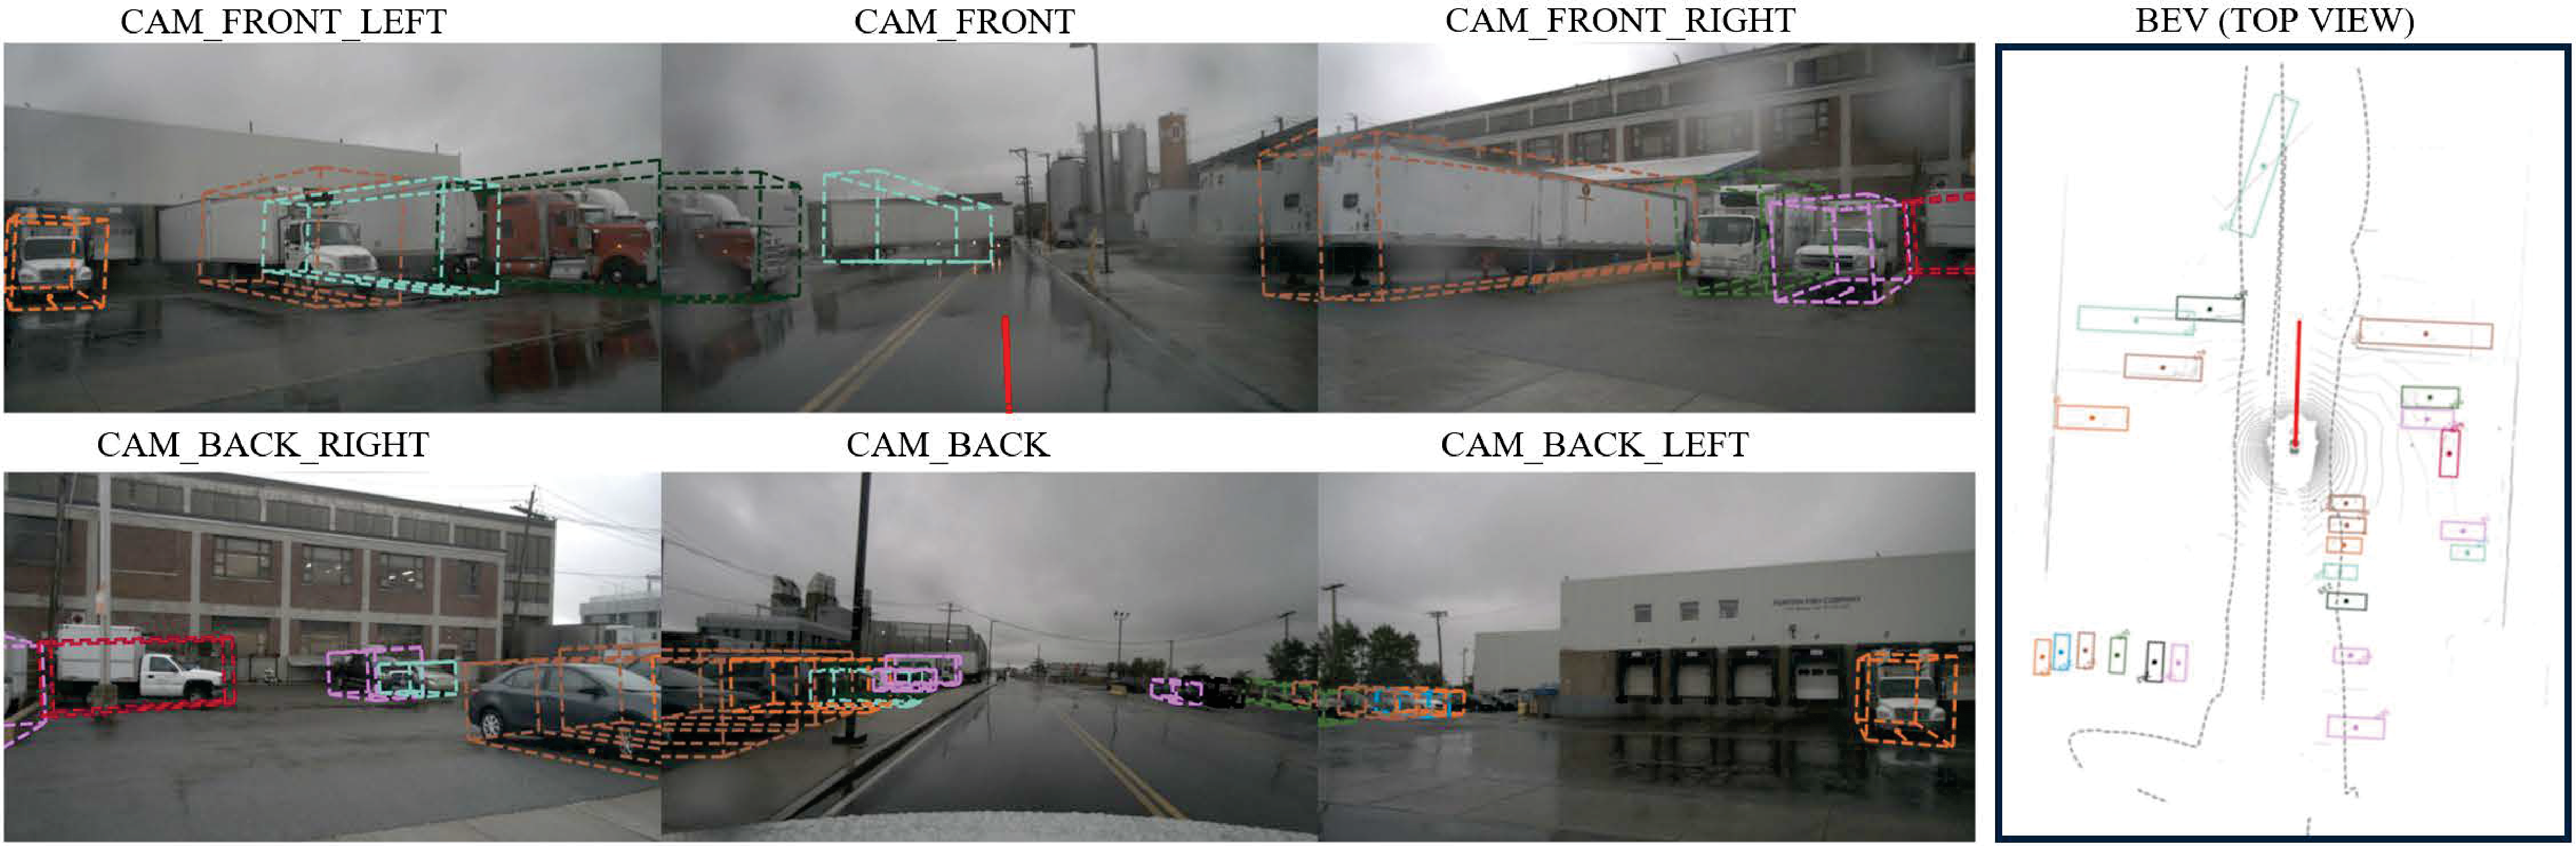
\includegraphics[width=1\linewidth]{Figures/supp_vis/fail_t1}
            \\
    ~
    \\
    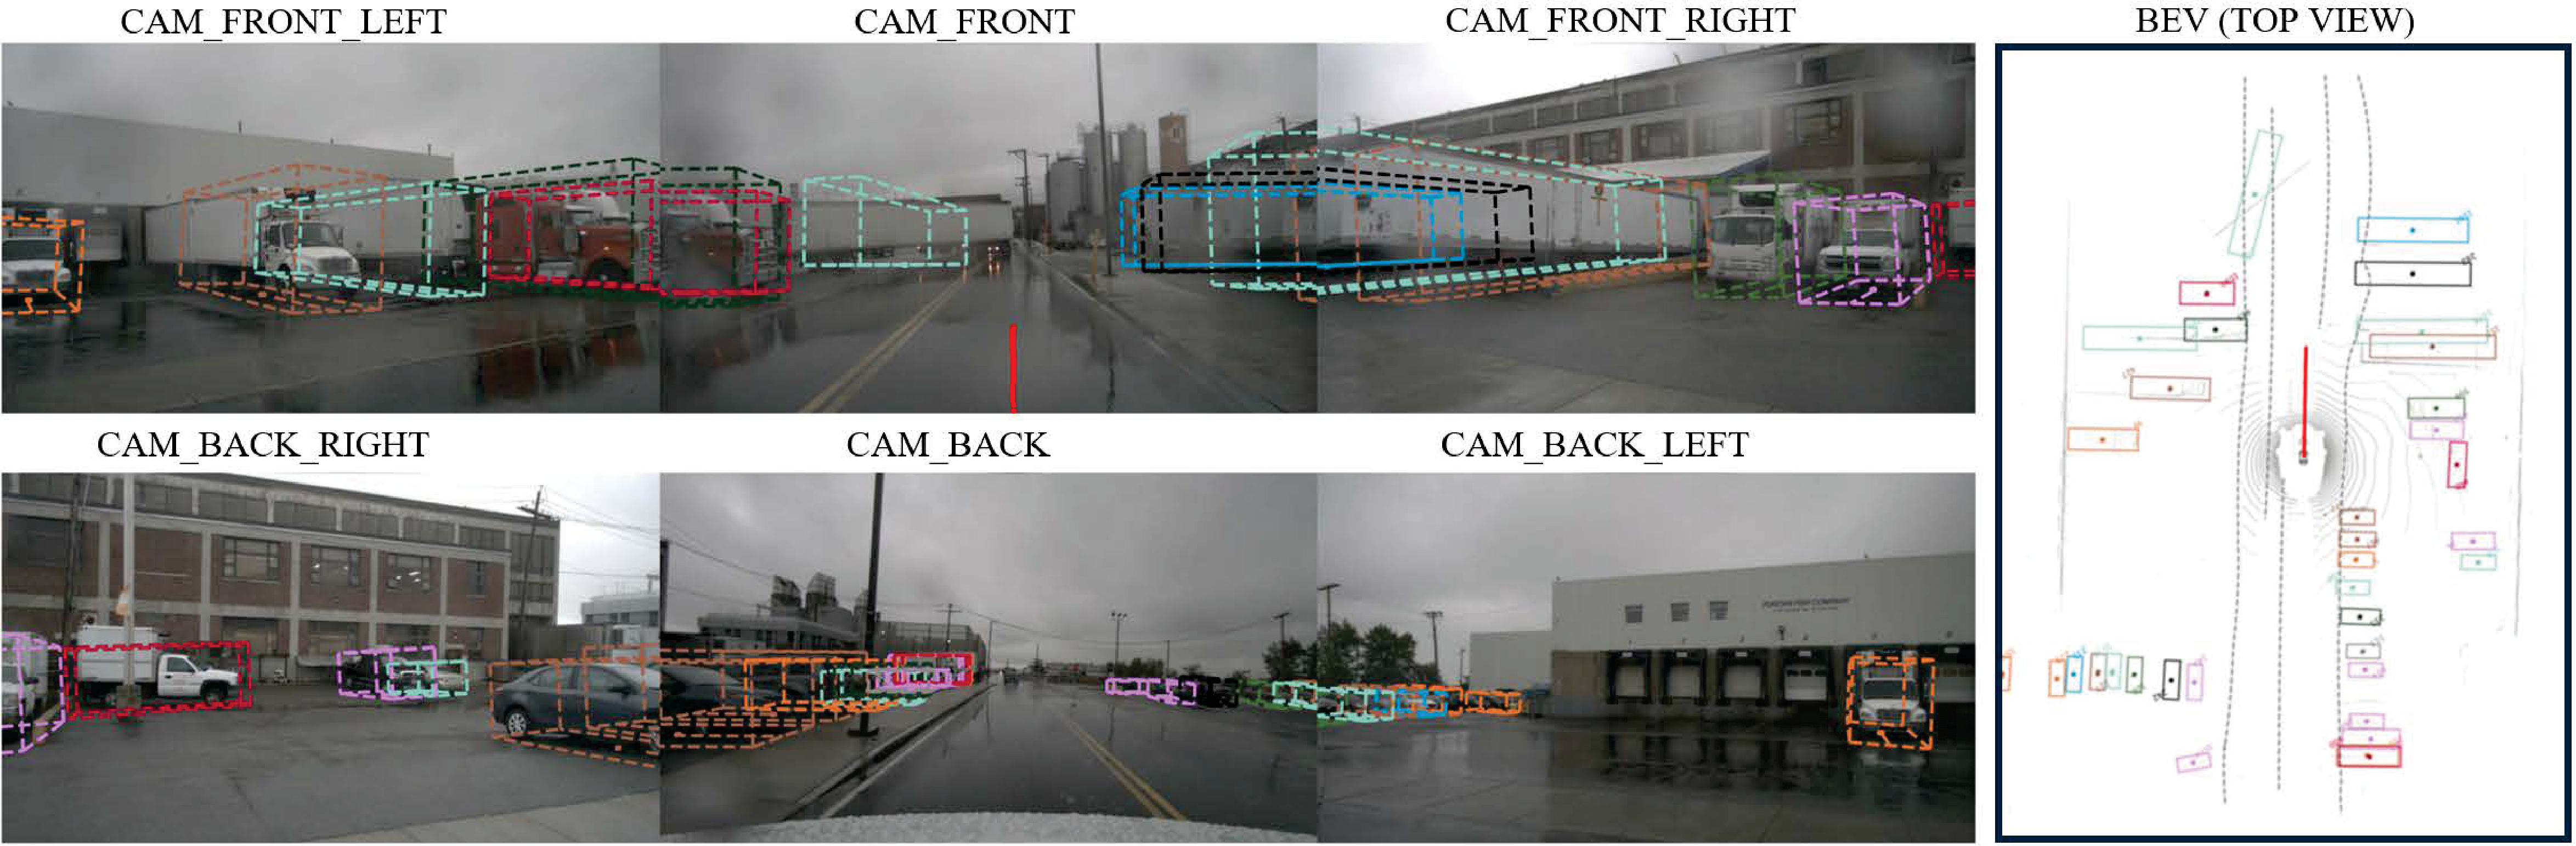
\includegraphics[width=1\linewidth]{Figures/supp_vis/fail_t2}
            \\
    ~
    \\
    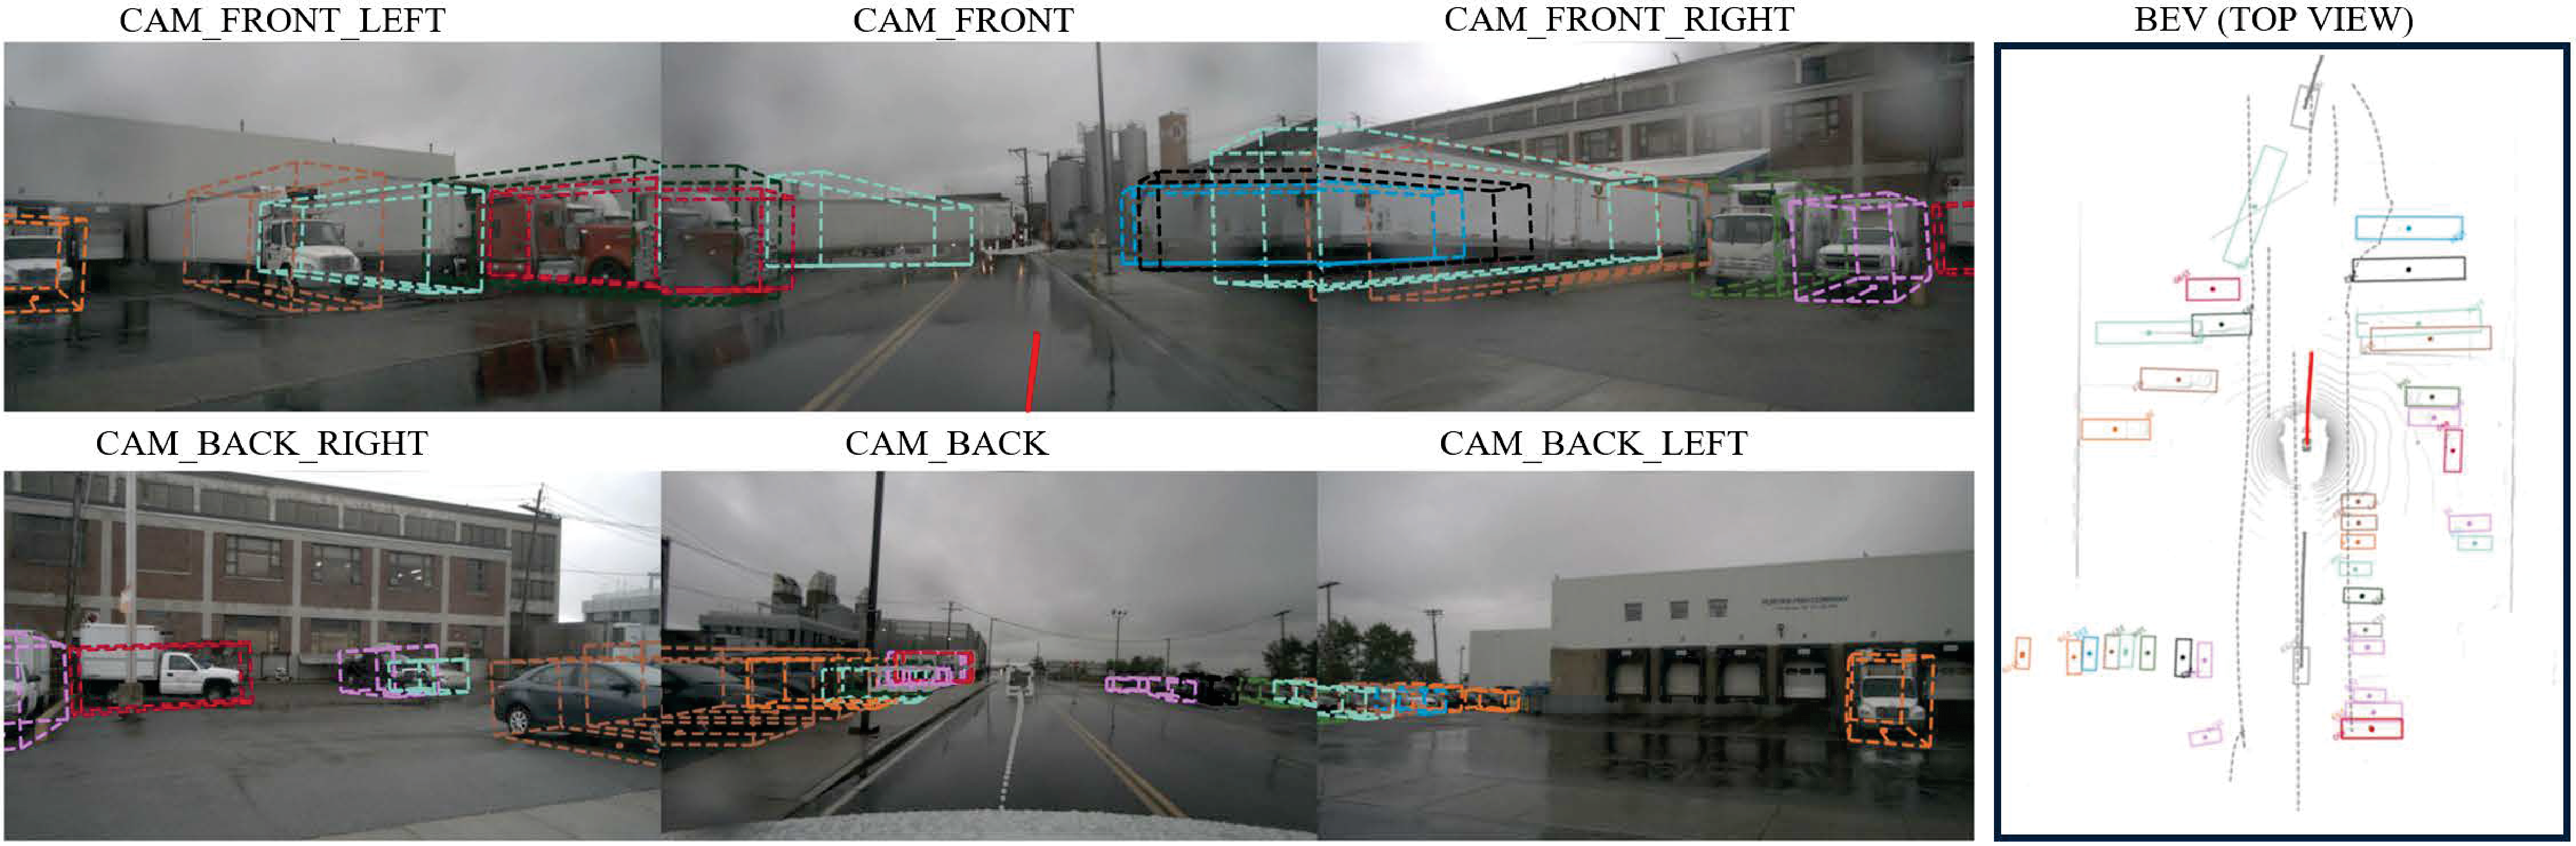
\includegraphics[width=1\linewidth]{Figures/supp_vis/fail_t3}

    \caption{失败案例。三行分别表示\model 在连续帧上的输出结果。可以看出，自车保持静止，但\model 仍提供了直行的规划结果。然而，从感知结果来看，在该场景中直行并非不合理的选择。这表明\model 未能充分利用自车的前一状态，导致与真实轨迹存在差异。}
    \label{fig:fail_vis}
  \end{figure}